\documentclass[12pt]{article}
\usepackage{../lecture}
\lecture{20}{Shortest Paths, DAG, and Floyd-Warshall}
\date{April 6, 2021}

\begin{document}
\maketitle

\section{The Crucial Optimality Substructure}

\subsection{Shortest Distance Problems}
\begin{itemize}
    \item The optimality substructure is $dist(s, u) = min_{v \in In(u)}(dist(s, v) + \ell(v, u))$.
    \item For Bellman-Ford, we used the formula $d(u) = \min_{v \in In(u)}(d(v) + \ell(v, u))$.
    \begin{itemize}
        \item If $v$ is on the shortest path of $u$ and $d(v) = dist(s, v)$, then $d(u) = dist(s, u)$ in the next iteration.
        \item We initialize $d(s) = 0$, and all $d(u) = \infty$ converges to the fixed point.
    \end{itemize}
    \item For Dijkstra, we used the formula $d(u) = \min_{v \in In(u), v \in X}(d(v) + \ell(v, u))$.
    \begin{itemize}
        \item $v$ in $X$ is known to have $d(v) = d(s, v)$.
        \item We only update $u$ adjacent to $X$. Each edge is only updated once.
        \item A good evaluation order saves a lot of work.
    \end{itemize}
    \item $dist(s, u) = \min_v(dist(s, v) + dist(v, u))$
    \begin{itemize}
        \item We would need to compute all $d(v, u)$ for all $v$, when we only need distance from $s$ in Bellman-Ford.
        \item This is a useful formula for computing all pair shortest distances in Floyd-Warshall.
    \end{itemize}
\end{itemize}

\section{Shortest Paths in DAGs}

\subsection{Single Source Shortest Path Problems}
\begin{itemize}
    \item \textit{Input}: A directed acyclic graph $G = (V, E)$ with arbitrary (including negative) edge lengths. For edge $e = (u, v)$, $\ell(e) = \ell(u, v)$ is its length.
    \begin{itemize}
        \item Given nodes $s, t$, find the shortest path from $s$ to $t$.
        \item Given node $s$, find a shortest path from $s$ to all other nodes.
    \end{itemize}
    \item We use Dijkstra's algorithm for non-negative edge lengths. The running time is $O(m + n\log n)$.
    \item We use the Bellman-Ford algorithm for arbitrary edge lengths. The running time is $O(mn)$.
    \item Simplication of algorithms for DAGs include no cycles and hence no negative length cycles, and that we can order nodes using topological sort.
\end{itemize}

\subsection{Algorithm for DAGs}
\begin{itemize}
    \item Suppose we want to find shortest paths from $s$. Let us ignore all nodes not reachable from $s$.
    \item Let $s = v_1, v_2, ..., v_{i}, ..., v_n$ be a topological sort of $G$.
    \item The shortest path from $s$ to $v_i$ cannot use any node from $v_{i + 1}, ..., v_n$.
    \item We can find the shortest paths in topological order.
    \item[] \lstinputlisting{code/dag-shortest-path.sudo}
    \item The shortest path DAG algorithm runs in $O(m + n)$ time.
\end{itemize}

\section{All Pairs of Shortest Paths}

\subsection{Shortest Path Problems}
\begin{itemize}
    \item \textit{Input}: A (undirected or directed) graph $G = (V, E)$ with arbitrary (including negative) edge lengths. For edge $e = (u, v)$, $\ell(e) = \ell(u, v)$ is its length.
    \begin{itemize}
        \item Find a shortest path for all pairs of nodes.
    \end{itemize}
    \item We could apply a single source $n$ times, once for each vertex.
    \begin{itemize}
        \item For arbitrary edge lengths, the runtime would be $O(mn^2)$, or $O(n^4)$ for $m \sim n^2$ (dense graphs).
        \item The space complexity would be $O(n^3)$.
        \item The algorithm is wasteful because the intermediate nodes can be any node. As a result, we compute the same path many times.
        \item Instead, we can try to restrict the set of intermediate nodes.
    \end{itemize}
\end{itemize}

\subsection{Recursion on the Index of Intermediate Nodes}
\begin{itemize}
    \item We can number the vertices arbitrarily as $v_1, v_2, ..., v_n$.
    \item $dist(i, j, k)$: the length of the shortest walk from $v_i$ to $v_j$ among all walks in which the largest index of an intermediate node is at most $k$ (could be $-\infty$ is there is a negative length cycle).
    \item[] \begin{center}
        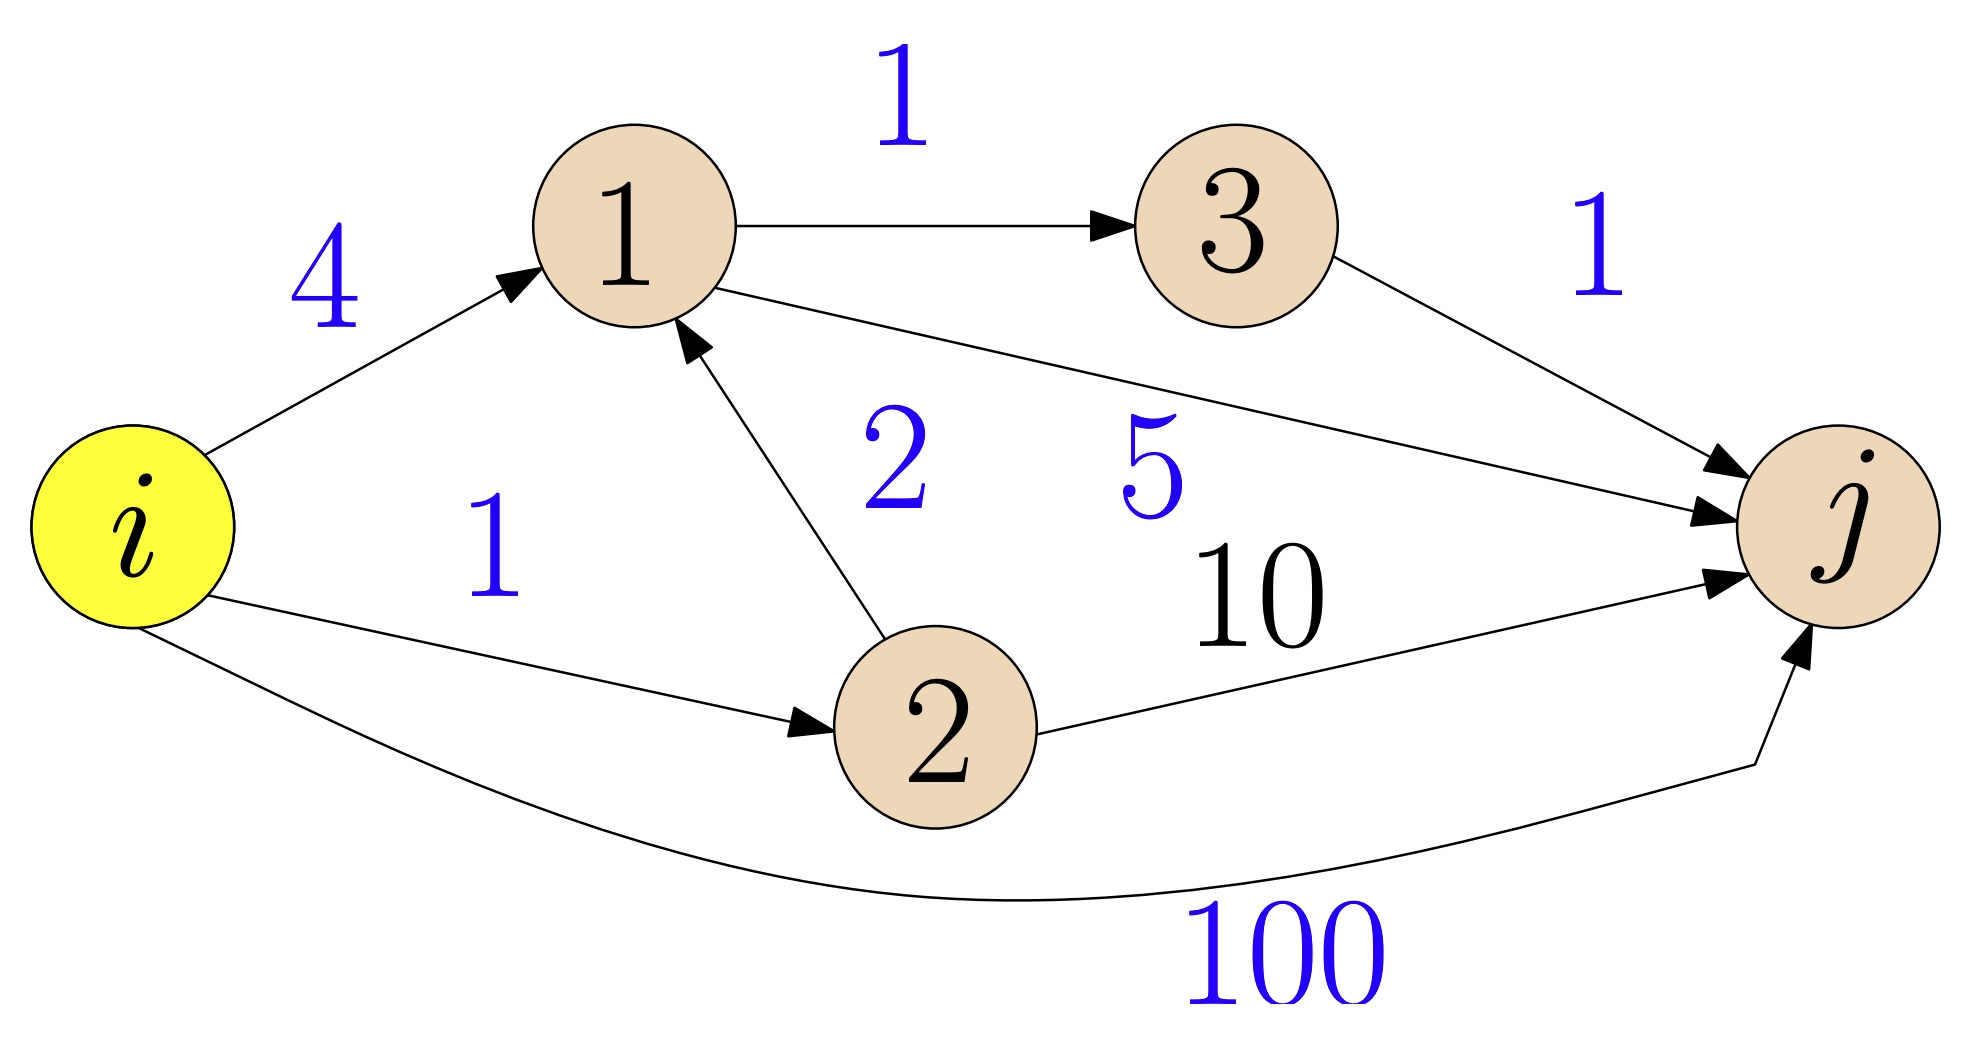
\includegraphics[width=0.75\textwidth]{images/all-pairs-dist-example.jpg}
    \end{center}
    \begin{itemize}
        \item $dist(i, j, 0) = 100$
        \item $dist(i, j, 1) = 9$
        \item $dist(i, j, 2) = 8$
        \item $dist(i, j, 3) = 5$
    \end{itemize}
    \item $dist(i, j, k) = \min \left\{
        \begin{tabular}{c}
            dist(i, j, k - 1) \\
            dist(i, k, k - 1) + dist(k, j, k - 1) \\
        \end{tabular}
    \right\}$
    \item[] \begin{center}
        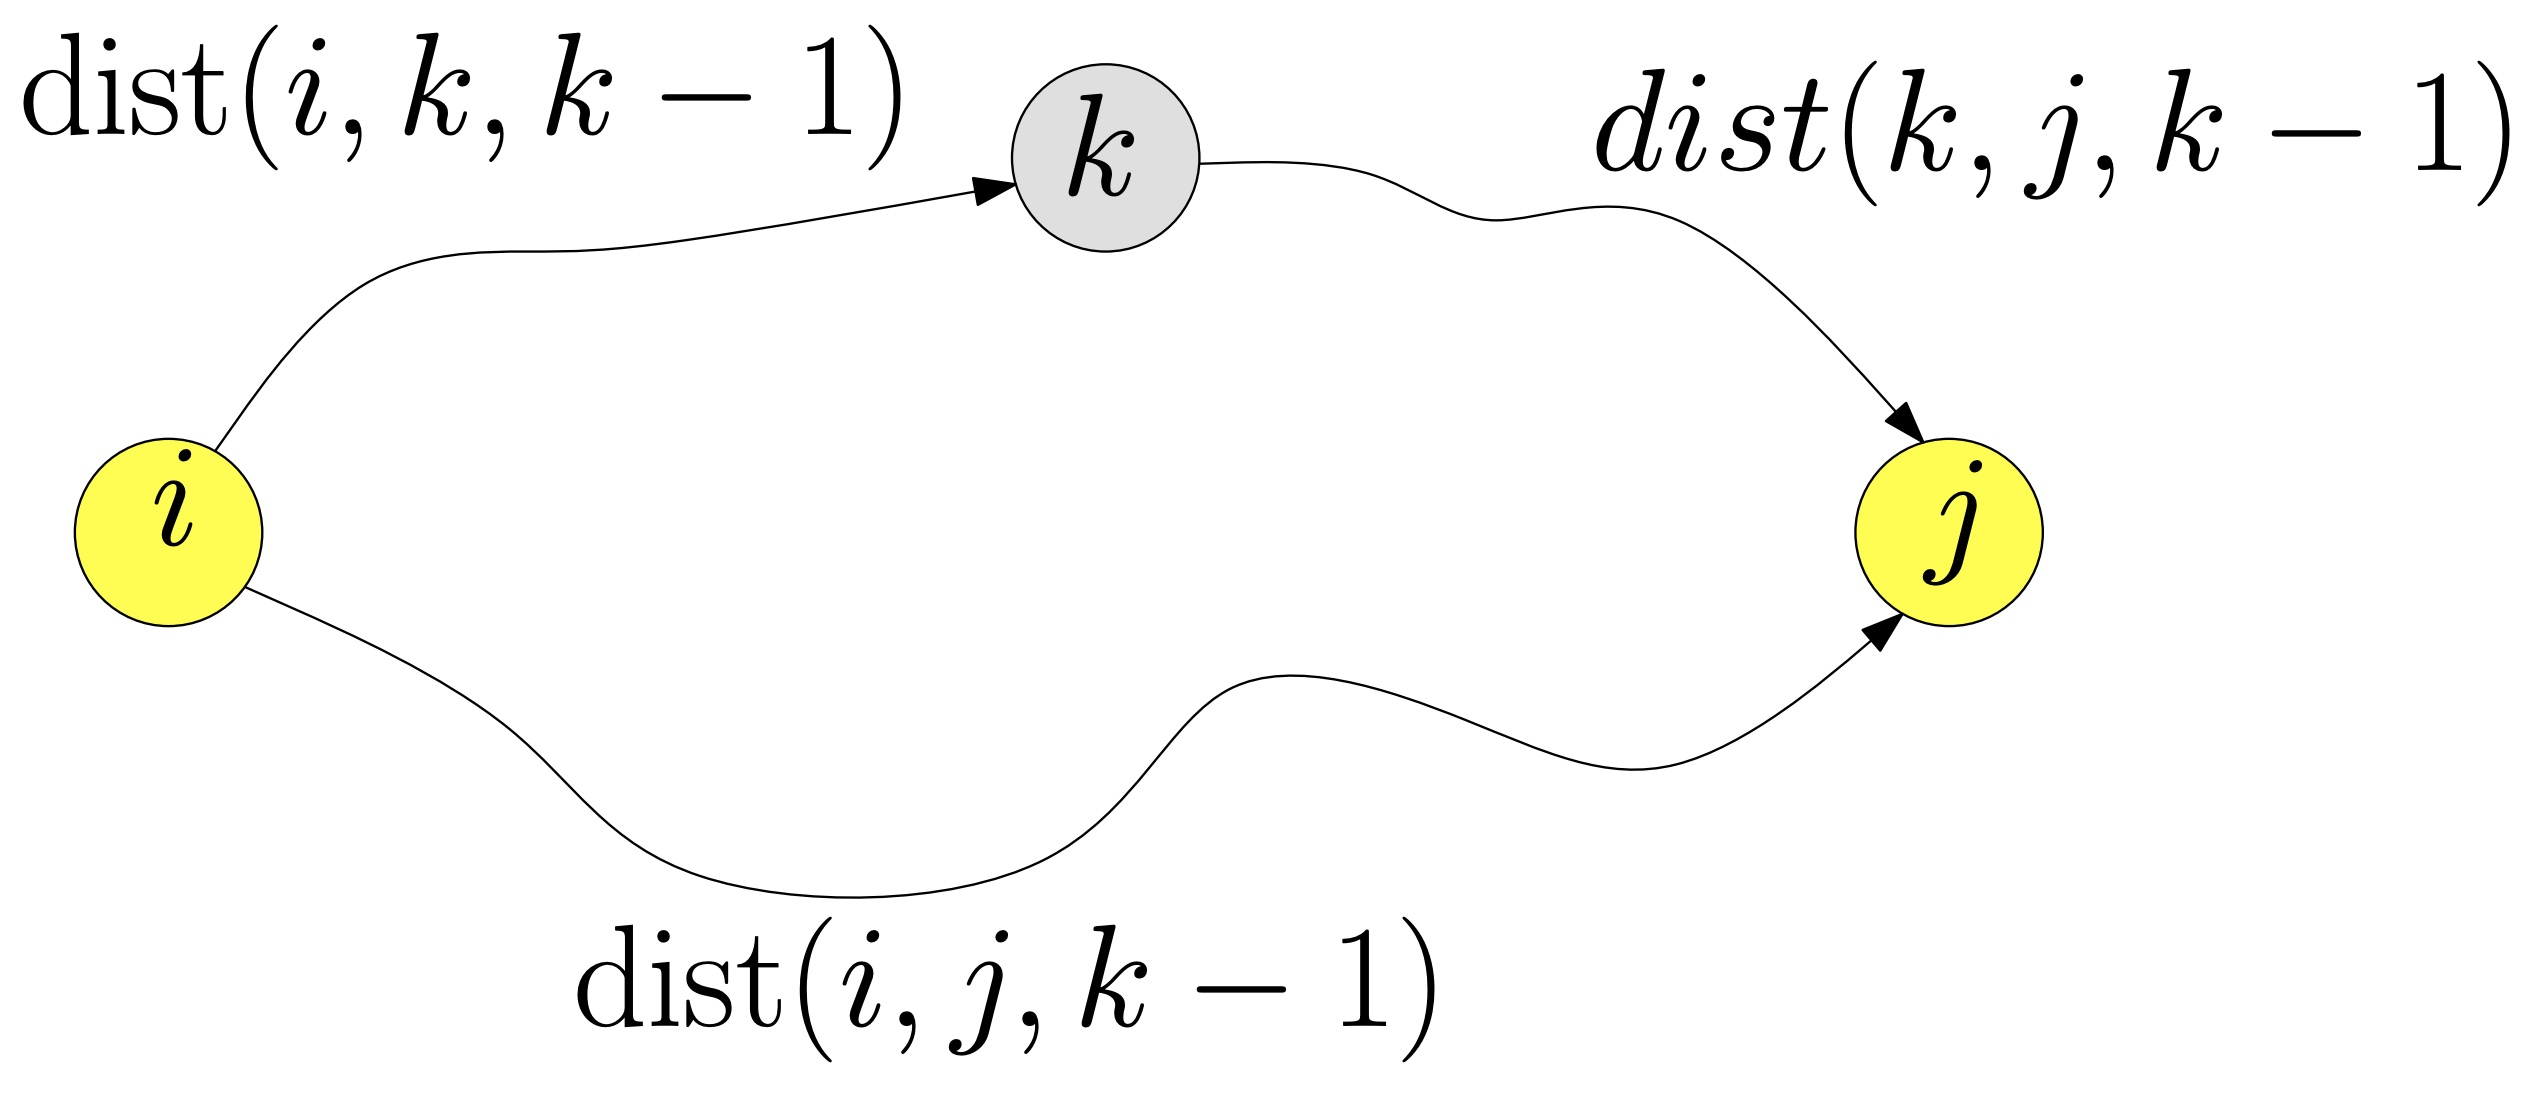
\includegraphics[width=0.5\textwidth]{images/all-pairs-recursive-example.jpg}
    \end{center}
    \item The base case is $dist(i, j, 0) = \ell(i, j)$ if $(i, j) \in E$, otherwise $\infty$.
    \item If $i$ can reach $k$, $k$ can reach $j$, and $dist(k, k, k - 1) < 0$, then $G$ has a negative length cycle containing $k$ and $dist(i, j, k) = -\infty$.
    \item The recursion is valid only if $dist(k, k, k - 1) \geq 0$. We can detect this during the algorithm or wait till the end.
    \item This gives us the Floyd-Warshall algorithm. The space complexity is $O(n^2)$ and the running time is $O(n^3)$.
    \item[] \lstinputlisting{code/floyd-warshall.sudo}
\end{itemize}

\end{document} 
